\documentclass[a4paper,UKenglish,cleveref, autoref, thm-restate]{lipics-v2019}

\usepackage{mathtools}
\DeclarePairedDelimiter\ceil{\lceil}{\rceil}
\DeclarePairedDelimiter\floor{\lfloor}{\rfloor}
%This is a template for producing LIPIcs articles. 
%See lipics-manual.pdf for further information.
%for A4 paper format use option "a4paper", for US-letter use option "letterpaper"
%for british hyphenation rules use option "UKenglish", for american hyphenation rules use option "USenglish"
%for section-numbered lemmas etc., use "numberwithinsect"
%for enabling cleveref support, use "cleveref"
%for enabling autoref support, use "autoref"
%for anonymousing the authors (e.g. for double-blind review), add "anonymous"
%for enabling thm-restate support, use "thm-restate"
%\graphicspath{{./graphics/}}%helpful if your graphic files are in another directory
\bibliographystyle{plainurl}% the mandatory bibstyle

\title{Computing Accumulated Delays in Real-Time Systems - A Summary} %TODO Please add


\author{Rajiv Alur}{University of Pennsylvania}{}{}{}

\author{Costas Courcoubetis}{Singapore University of Technology and Design}{}{}{}

\author{Thomas A. Henzinger}{IST Austria}{}{}{}

\ccsdesc[500]{Theory of computation~Timed and hybrid models}

\keywords{Timed Automata, Duration Bounded Reachability, Region graph, Bound-Labeled Graph, Bound expressions} %TODO mandatory; please add comma-separated list of keywords

\nolinenumbers %uncomment to disable line numbering

\hideLIPIcs  %uncomment to remove references to LIPIcs series (logo, DOI, ...), e.g. when preparing a pre-final version to be uploaded to arXiv or another public repository

\authorrunning{R. Alur, C. Courcoubetis, T.A. Henzinger}

\begin{document}

\maketitle
\medskip
This is a summary of the paper written as a fulfillment of the course Timed Automata at\textbf{ Chennai Mathematical Institute, India} instructed by \textbf{Prof. B. Srivathsan} and submitted by \textbf{Soumodev Mal} on \today.

\begin{abstract}
The objective of the paper is to find an optimal PSPACE verification algorithm for \textbf{duration bounded reachability problem} of real time systems. The paper uses Timed Automata to model real-time systems.\\
The \textbf{duration bounded reachability problem} w.r.t. timed automata is the question whether there exists a run of the automaton starting from an initial state to a final state whose \textbf{duration} satisfies an arithmetic constraint.\\
The \textbf{duration of a run} can be seen as a linear combination of the timed spent in each state visited through the run.
\end{abstract}

\section{MOTIVATION}
\label{sec:mot}
Model checking in Computer Science is a method for checking whether a finite-state model of a system meets a given specification. In the past 30-40 years, Model checking has emerged as a powerful tool for verification of such finite-state models(FSMs) and incorporated into several extensions of FSMs.\\
One such extension is Real-time Systems, i.e., Finite-state models with timings.\\
While properties that are continuous w.r.t. time can be verified easily using Real-time temporal logic, Verifying properties that are \textit{possibly intermittent} is not easily verifiable and that is the main motivation of the paper. The latter properties are known as duration bounded causality properties while the former are known as time-bounded causality properties.
\section{SUMMARY}
\subsection{Preliminaries}

The paper takes the formalism of Timed Automata in order to model Real-Time Systems.\\
According to the paper, A Timed Automata $A$ is a three tuple $(S,X,E)$ where,
\begin{itemize}
\item $S$ is a finite set of \textit{locations}
\item $X$ is a finite set of clocks
\item $E$ is a finite set of transitions of the form $(s,t,\varphi,x)$ where
\begin{itemize}
\item $s \in S$ is a source location
\item $t \in S$ is a target location
\item $\varphi$ are clock constraints that are positive boolean combination of formulas of the form: $y<k\ or\  y>k\ or\  y=k$ where $y \in X$ and $k \in \mathbb{N}$
\item $x \in X$ is a clock that is reset. [Note: This doesn't affect the expressiveness of the Timed Automata. Why?]
\end{itemize}
\end{itemize}
\smallskip
A State $\sigma$ of $A$ is a tuple $(s,c)$ where $s \in S$ and $c \in \mathbb{R}^X$ is a clock valuation that assigns a non-negative real number to each clock.[Note: The state space $\Sigma$ is infinite]\\
A run of a Timed Automata is an alternating sequence of Transition successor and time successor where
\begin{itemize}
\item Transition successors are instantaneous transition from one state to another allowing only a single reset
\item Time successors elapses time and remains in the same state.
\smallskip
\end{itemize}
The main problem to address the time-bounded reachability problem for the Timed Automata(as defined) is that there are infinitely many states. The standard method to solve this problem is by categorizing states into finitely many regions using some equivalence relation $\cong$ such that $[ \sigma ]_{\cong} \subseteq \Sigma$ is an equivalence class and establishing relations between those equivalence classes.\\
A Stable Equivalence Relation: $[\sigma]_{\cong} \rightarrow [\tau]_{\cong}\ \iff\  \forall \sigma' \in [\sigma]_{\cong}\ \exists \tau' \in [\tau]_{\cong}: \sigma' \rightarrow \tau'$.\\
A Back Stable Equivalence Relation: $[\sigma]_{\cong} \rightarrow [\tau]_{\cong}\ \iff\ \forall \tau' \in [\tau]_{\cong}\ \exists \sigma' \in [\sigma]_{\cong}: \sigma' \rightarrow \tau'$.\\
A Region graph is a graph with vertices as region equivalence classes defined below:
Two states $(s,c)$ and $(t,d)$ are region equivalent $\approx$ iff :
\begin{itemize}
\item s=t
\item for each clock $x \in X$, either $\floor{c(x)}\footnote{integral part of c(x)}=\floor{d(x)}$ or both $c(x)> m_x\footnote{the maximum constant in the constraints $\varphi$}\ and\ d(x)>m_x$
\item for each clock $x,y \in X$,$\overline{c(x)}\footnote{the fractional part of c(x)}<\overline{c(y)} \iff$ $\overline{d(x)}<\overline{d(y)}$.
\item for each clock $x \in X$,$\ \overline{c(x)}=0 \iff\overline{d(x)}=0$. 
\end{itemize}
[Note: The region equivalence relations $\approx$ are both stable as well as back-stable.]\\
A region R is a boundary region iff there exists some x for which $\overline{x}=0$ and an open region otherwise.\\
The number of regions are bounded by $|S|.2^n.n!.\Pi_{x \in X} (m_x+1)$.\\
The edges of the region graph are of two types:
\begin{itemize}
\item Transition edges are instantaneous transition from one region to another (by changing state)
\item Time edge elapses time and for each boundary region R, there is an edge from \textit{pred(R)}\footnote{pred(R) is an open region Q such that $\exists (s,c) \in Q \rightarrow^{\delta} (s,c+\delta) \in R$ and $\forall\ non\ neg\ \epsilon < \delta\ (s,c+\epsilon) \in Q$} and an edge to \textit{succ(R)}\footnote{succ(R) is an open region Q' such that $\forall (s,c) \in Q' \rightarrow^{\delta} (s,c-\delta) \in R$ and $\forall\ non\ neg\ \epsilon < \delta\ (s,c-\epsilon) \in Q'$}
\smallskip
\end{itemize}
Thus, the region graph makes the state space finite and hence we are able to decide the time-bounded reachability problem but it is still not enough to address the duration-bounded reachability problem.Thus, in the next section, we look at a construct that would help us constrain the accumulated satisfaction times of state predicate or in other words, constraints over accumulated time that are not continuous.

\subsection{Duration-bounded Reachability}
For a Timed Automata $A$, \textit{duration measure} is a function $p : s \rightarrow i$ where s is a location in A and i is a non-negative integer. The \textit{duration constraint} for A is the integral $\int p \in I$ where p is a duration measure and I is the bounded interval of a non-negative real line whose endpoints are integers.[Note: I can be closed,half-closed or open].\\
In order to address the duration-bounded reachability problem, we need to keep track of the accumulated time at each state of a run in A. To do so we extend the state space of $A$ to evaluate the duration constraint along the runs of A. Thus, an extended state of A is a pair $(\sigma,\epsilon)$ where $\sigma$ is a state of A and $\epsilon$ is a non-negative real number.\\
The successor relation of the extended state is as follows:
\begin{itemize}
\item Transition successors are instantaneous transition from one extended state $(s,c,\epsilon)$ to another $(t,c[x:=0],\epsilon)$ allowing only a single reset with no change in duration constraint
\item Time successors elapses time $\delta$ and remains in the same state and the duration constraint $\epsilon$ updated as $\epsilon + p(s).\delta$
\smallskip
\end{itemize}
We formally define the duration-bounded reachability problem by the tuple $(A,R_0,R_f,\int p \in I)$ where A is a Timed Automata, $R_0$ and $R_f$ are regions and p is the duration measure. It asks:\\
\textbf{"Given two regions $R_0$ and $R_f$ of a timed automaton A, and a duration constraint $\int p \in I$ for A, is there a state $\sigma \in R_0$, a state
$\tau \in R_f$, and a non negative real $\delta \in I$ such that $(\sigma,0)\rightarrow^* (\tau,\delta)$?"}\\
For the extended automaton, we are again left with the same problem we encountered, that is, the state space becomes infinite again that restrains us from deciding reachability. To address the issue, a similar approach is taken of categorizing the extended states into finitely many bound-labeled regions(which we'll see in the following section).

\subsection{A Solution to Duration-bounded Reachability}
We extend the region graph to an infinite graph with vertices of the form $(R,L,l,U,u)$ known as Bound-labeled region where R is a region, L and U are linear expressions over the clock variables, and l, u are boolean values.\\
The bound expressions L and U are functions over the current clock valuation $c$ and is basically the infimum and the supremum of the possible values of $\int p$ in moving from $(s,c) \in R$ to a region $R_f$\footnote{$R_f$ is  a special vertex without any outgoing edge and denotes the final region}.The bit l = 0 denotes the infimum to be open interval and l=1 denotes closed interval. Similarly, u=0 denotes the supremum to be open and u=1 denotes closed interval.\\
The Bound expressions have a special form.
\begin{figure}[h]
\centering
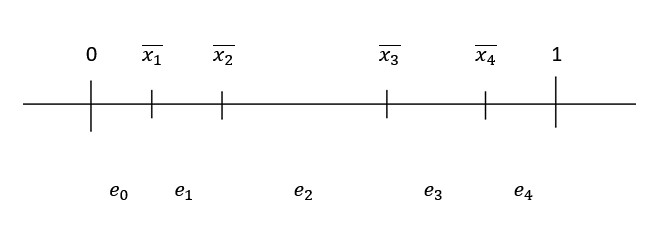
\includegraphics[scale=.4]{exp}
\end{figure}
Let the clocks be ordered as $0 \leq \overline{x_1} \leq \overline{x_2}\leq ... < \overline{x_n} < 1$, the expression $e_i$ can be written as $\overline{x_{i+1}} - \overline{x_i}$ [see fig. above] for $0<i<n$ and $e_0 = \overline{x_1}$ and $e_n = 1 - \overline{x_n}$.
Thus, a bound expression is a positive linear combination of the expressions $e_0,e_1,...,e_n$, i.e., $a_0.x_0 +...+a_n.x_n$ where $a_0,...,a_n$ are non-negative integer constants. The Bound expression can be written as $(a_0,a_1,...,a_n)$.\\
Now, construct $\mathcal{B}_{p,R_f}(A)$, the bound graph of A for the duration measure p and the final region $R_f$.The vertices are bound-labeled regions and $R_f$. The edges are defined below:\\
Suppose $(R,L,l,U,u) \rightarrow (R',L',l',U',u')$ with duration measure of R as $a$, $L=(a_0,a_1,...,a_n)$, $L'=(a_0,'a_1',...,a_n')$, $U=(b_0,b_1,...,b_n)$ and $U'=(b_0',b_1',...,b_n')$. \\
\textbf{Time edges} 
\begin{itemize}
\item When R is an open region and R' is a boundary region where $R=pred(R')$. Let $1\leq k \leq n$ be the largest index where R' satisfies $\overline{x_k} = 0$, then,
\begin{itemize}
\item $\forall\ 0 \leq i \leq n-k,\ a_i = a'_{i+k}$ and $b_i = b'_{i+k}$
\item $\forall\ n-k \leq i \leq n,\ a_i = 0$ and $b_i = 0$
\item $a_n = a_k' + a$ and $b_n = b_k' + a$
\item $l=l'$ and $u=u'$
\end{itemize}
\begin{figure}[h]
\centering
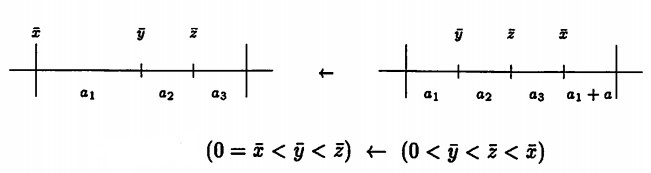
\includegraphics[scale=.4]{2}
\end{figure}
\end{itemize} 

\begin{itemize}
\item When R is a boundary region and R' is an open region where $R'=succ(R)$.
\begin{itemize}
\item $\forall\ 0 \leq i \leq n,\ a_i = a'_{i}$ and $b_i = b'_{i}$
\item $a_0 = 0$ and $b_0 = 0$
\item $l=l'$ and $u=u'$
\end{itemize}
\begin{figure}[h]
\centering
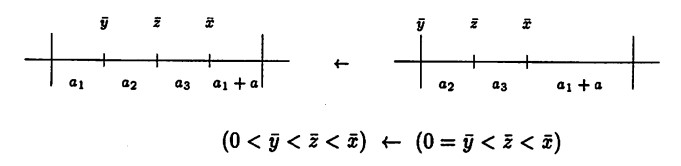
\includegraphics[scale=.4]{1a}
\end{figure}
\end{itemize} 

\textbf{Transition edges} 
\begin{itemize}
\item When R is an open region and R' is a boundary region. Let $1\leq k \leq n$ be the smallest fractional part where $x_k$ is reset in R, then,
\begin{itemize}
\item $\forall\ 0 \leq i < k,\ a_i = a'_{i+1}$ and $b_i = b'_{i+1}$
\item $\forall\ k \leq i < n,\ a_i = a_i'$ and $b_i = b_i'$
\item $if\ a_n' \leq a_1' + a$ then $a_n=a_n'$ else $a_n = a_1' + a$
\item $if\ b_n' \geq b_1' + a$ then $b_n=b_n'$ else $b_n = b_1' + a$
\item $if\ a_n' > a_1' + a$ and $a>0$ then $l=1$ else $l=l'$
\item $if\ b_n' < b_1' + a$ and $a>0$ then $u=1$ else $u=u'$
\end{itemize}
\begin{figure}[h]
\centering
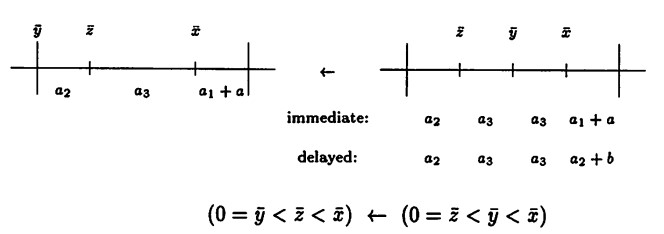
\includegraphics[scale=.4]{1b}
\end{figure}
\end{itemize} 

\begin{itemize}
\item When both R and R' are a boundary regions and Let $1\leq k \leq n$ be the smallest fractional part where $x_k$ is reset in R, then,
\begin{itemize}
\item $\forall\ 0 \leq i < k,\ a_i = a'_{i+1}$ and $b_i = b'_{i+1}$
\item $\forall\ k \leq i < n,\ a_i = a'_{i}$ and $b_i = b'_{i}$
\item $l=l'$ and $u=u'$
\end{itemize}
\begin{figure}[h]
\centering
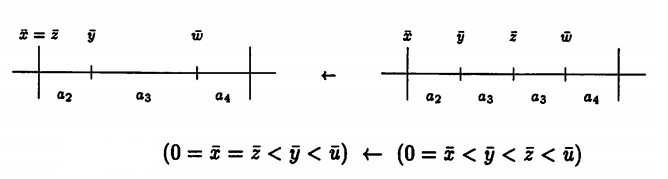
\includegraphics[scale=.4]{3}
\end{figure}
\end{itemize}

This completes the definition of Bound-labeled graph $\mathcal{B}_{p,R_f}(A)$.

\subsection{Reachability in Bounds Graph}
Given a timed Automata A, with duration measure p, and $R_f$ as final region, From any state in the bounds graph $R_f$ is reachable iff there is a path to $R_f$ from a bounded labeled region.\\
The above claim can be proved by induction on the length of the run using the definition of edges in the bounds graph. Since, using the back stable property of the transition edges, we can start from the final region and traverse backwards in a breadth first fashion in order to check reachability. Since there are infinitely many distinct bounds expressions, we can't say if the search would terminate or not.\\
In the next section, we see that the search would eventually terminate.

\subsection{Collapsing the Bounds Graph}
We will observe that after a non-negative integer $m$, the coefficient of the bound expressions becomes irrelevant w.r.t. I.\\
We define an equivalence relation $\cong_m$ over bound-labeled regions as follows:\\ For non-negative integers a and b,
a $\cong_m$ b iff either a=b or (a>m and b>m).\\ For two bound expressions $e =(a_0,a_1,...,a_n)$ and $f=(b_0,b_1,...,b_n)$, e $\cong_m$ f iff for all i, $a_i \cong_m b_i$.\\
For two Bound-labeled regions $B_1 \cong_m B_2$ iff :
1)$R_1=R_2$, 2) $L_1 \cong_m L_2, U_1 \cong_m U_2$, 3)either $l_1=l_2$ or some coefficient in $L_1 > m$, 4) either $u_1=u_2$ or some coefficient in $U_1 > m$.\\
But now we cannot ensure that equivalence relation $\cong_m$ is back-stable.\\
But it turns out to be back-stable by the following lemma.\\
\textit{If the bounds graph contains an edge from a bound-labeled region $B_1$ to $B_1'$ and $B_1' \cong_m B_2'$ then $\exists B_2$ such that $B_1 \cong_m B_2$ and there is an edge from $B_2$ to $B_2'$.}\\
Now since the equivalence relation is back-stable, to check reachability of bound-labeled regions, we can just look at the quotient graph $[\mathcal{B}_{p,R_f}(A)]_{\cong_m}$.\\
Now to get an upper bound on the constant $m$ for solving duration bounded reachability, they basically use the concept of max-constant as seen in the region graphs.\\
A bound expression e is $m-constrainted$ iff all the coefficient in e are atmost m+1. For every bound expression e, there is a unique m-constrained bound-expression $\gamma(e)$ such that $e \cong_m \gamma(e)$.
They extend this concept of m-constrained to Bound-labeled Regions restricting l=0 or u=0 if some coefficient of L or U is m+1 where L and U are m-constrained.\\
So for all bound-labeled regions there is a unique m-constrained bound-labeled region. This implies that every $\cong_m$-equivalence class contains exactly one m-constrained bound-labeled region.\\
The number of m-constrained expressions over n clocks are $(m+2)^{n+1}$. Because the constrains ranges from  0 to m+1 and there are n+1 expressions for n clocks.
Thus for a given region R,the number of m-constrained bound-labeled regions is $4.(m+2)^{2(n+1)}$. Because l and u can have the values 0 or 1 each and there are two bound expressions U and L. From the bound on the clock region, we get the bound on the number of m-constrained bound-labeled regions of A, i.e.,\\
$$4.|S|.n!.2^{n+2}.(m+2)^{2(n+1)}.\Pi_{x\in X}(m_x+1)$$
Hence, when constructing, in a backward breadth-first fashion, the portion of the bounds graph from which the special vertex $R_f$ is reachable, we need to explore only m-constrained
bound-labeled regions. For each m-constrained bound-labeled region B, we first construct all
predecessors of B. The number of predecessors is finite, and corresponds to the number
of predecessors of the clock region of the predecessors in the region graph. Each predecessor
that is not an m-constrained bound-labeled region is replaced by the $\cong_m$-equivalent m-constrained
region. The duration-bounded reachability property holds if a bound-labeled region B with
$I(B) \cap I=\emptyset$\footnote{I(B) is the bounded interval w.r.t. the bound-labeled region B} is found. If the search terminates otherwise, by generating no new m-constrained bound-labeled regions, then the answer to the duration-bounded reachability problem is negative.
The time complexity of the search is proportional to the number of m-constrained bound-labeled
regions. The space complexity of the search is Pspace, because the representation of an m-constrained bound-labeled region and its predecessor computation requires
only space polynomial in the length of the problem description.\\
Thus the duration bounded reachability problem for Timed Automata is in PSPACE since the unbounded reachability is PSPACE hard for clock regions.

\section{CONCLUSION}
The solution to the Duration bounded reachability problem is given w.r.t. some initial and final region. But this can be replaced by specific states with rational values or by a specific location. Thus the PSPACE solution can be extended to rational states.\\
An interesting fact: Instead of putting duration measures in Timed Automata, a more general approach extends the timed automata with variables that measure accumulated durations. These variables are called integrators or stopwatches which can be reset or constrained.However, it's reachability is undecidable.
In constrast, instead of giving such power directly to the automaton, the problem was solved when the duration constraints were treated separately from the system as properties,i.e., the specification language was strengthened.
\subsection{Open Problems}
The expressiveness of specification languages can be increased further. For example,
it is possible to define temporal logics with duration constraints or integrators. The decidability
of the model-checking problem for such logics remains an open problem.
\end{document} 
